\documentclass{article}
\usepackage[utf8]{inputenc}
\usepackage{graphicx}
\usepackage{float} 
\usepackage{array}
\textheight 24cm
\textwidth 16cm
\oddsidemargin 0cm
\evensidemargin 0cm
\topmargin 0cm
\hoffset -0mm
\voffset -20mm
\usepackage[]{listings}
\usepackage{amsmath}
\title{Geometric Modeling}
\author{Manuel Camargo & Mohamed Traoré &  Nicolas Gindrier}
\date{}
\begin{document}

\maketitle
\section*{Summary and presentation}
\begin{figure}[H]
   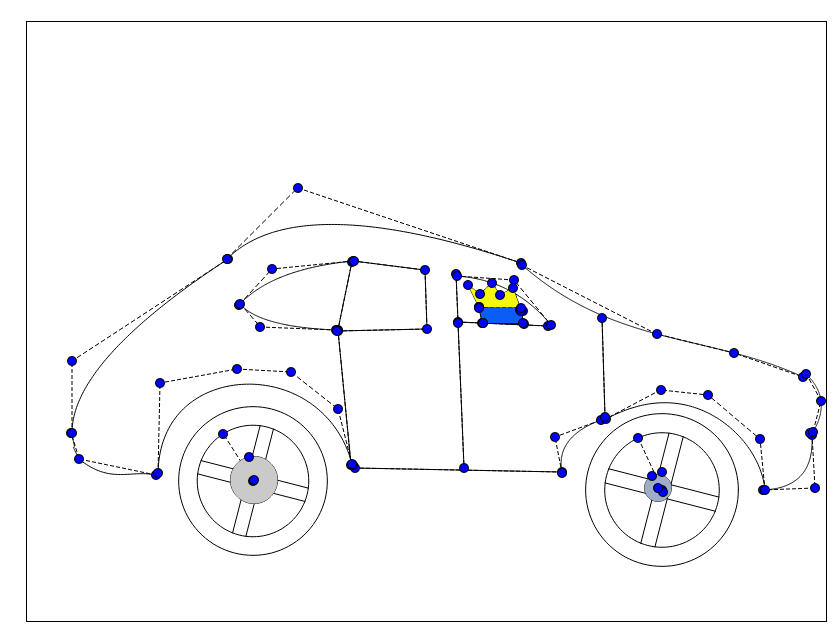
\includegraphics[scale = 0.5]{Pictures/narutovoiture.png}
\end{figure}
\section*{Organization}
We used Github.
\section*{Curves}
\subsection*{Curves 1-D}
\subsection*{Curves 2-D}
\subsubsection*{Bezier-Aitken}
These both curves are coded from the same way. A recursive function on the contrrol points is called. We store points in a static tab and we linked these points after. It is also used for \textit{Hermite1} and \textit{Hermiteclosed}. For \textit{Aitken} we use a uniform parameterization. 
\begin{figure}[H]
   \includegraphics[scale = 0.5]{Pictures/bezier-aitken.png}
\end{figure}
\subsubsection*{Hermite1-Hermite closed}
These curves are made with some Hermite cubic splines, based on P1, P2 and their tangent. That allows to have $C^1$ closed curves. The difficulty is to impose good direction, weight and sense for tangents. %From nico to nico explain formulas   + scheme of projection
\begin{figure}[H]
   \includegraphics[scale = 0.5]{Pictures/hermite.png}
\end{figure}
\subsubsection*{Wheel-Gear}
It is not really curves. The goal here is to play with the variable \textit{frame}. We are midway between cartoon and CAD.\\
In both cases \textit{frame} is traduced as rotation speed. \\
For \textit{Wheel} we draw two circles. We use the points of the little circle.%from nico to nico explain
For gear %from nico to nico explain + scheme of angles
\begin{figure}[H]
   \includegraphics[scale = 0.5]{Pictures/gear-wheel.png}
\end{figure}

\subsection*{others} %for example DelCurve
\section*{Prospects}
We had a lot of ideas but some of them have not been made. It was because of timme, or because we fear to modify some files. We do not master the architecture of the whole project. For example matstering scene.h would allowed many things, like to save. 
\end{document}
